\documentclass[12pt]{article}
\usepackage{amsmath}
\usepackage{tikz}
\usepackage{tikz-3dplot}
\usetikzlibrary{calc,3d,decorations.markings, backgrounds, positioning,intersections,shapes}
\usepackage{pgfplots}

\newcommand{\InterSec}[3]{%
  \path[name intersections={of=#1 and #2, by=#3, sort by=#1,total=\t}]
  \pgfextra{\xdef\InterNb{\t}}; 
}


 \newcommand\getEquator[2]
  {
    \def\yt{#1}
    \def\zt{#2}

    \pgfmathsetmacro{\betav}{acos(\zt)};

    \def\gammav{0}
    \ifthenelse{\equal{\betav}{0.0}}
    {
      \def\alphav{0}
    }
    {
      \pgfmathsetmacro{\alphav}{asin(\yt/(sin(\betav))}
    };
  }


   % to color a line
        \tikzset{test/.style={
          postaction={
            decorate,
            decoration={
              markings,
              mark=at position \pgfdecoratedpathlength-0.5pt with 
              {\arrow[blue,line width=#1] {>}; },
              mark=between positions 0 and \pgfdecoratedpathlength step 0.5pt with {
                \pgfmathsetmacro\myval{multiply(divide(
                  \pgfkeysvalueof{/pgf/decoration/mark info/distance from start}, 
                \pgfdecoratedpathlength),100)};
                \pgfsetfillcolor{blue!\myval!green};
                \pgfpathcircle{\pgfpointorigin}{#1};
                \pgfusepath{fill};}
              }
            }
          }
        }




\begin{document}
\begin{center}
	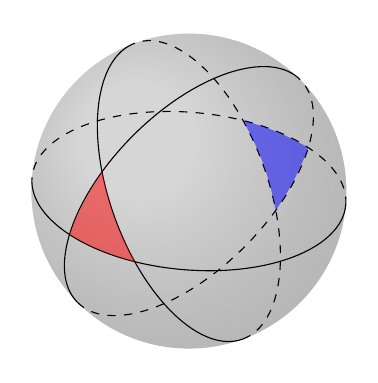
\begin{tikzpicture}

		\pgfmathsetmacro\R{2}
		\fill[ball color=white!10, opacity=0.2] (0,0,0) circle (\R); % 3D lighting effect



		\foreach \angle[count=\n from 1] in {-5,225,290} {

				\begin{scope}[rotate=\angle]
					\path[draw,dashed,name path global=d\n] (2,0) arc [start angle=0,
							end angle=180,
							x radius=2cm,
							y radius=1cm] ;
					\path[draw,name path global=s\n] (-2,0) arc [start angle=180,
							end angle=360,
							x radius=2cm,
							y radius=1cm] ;
				\end{scope}
			}
		\InterSec{s1}{s2}{I3} ;
		\InterSec{s1}{s3}{I2} ;
		\InterSec{s3}{s2}{I1} ;
		%
		\fill[fill=red,opacity=0.5] (I1) to [bend right=8.5]  (I2) to [bend left=7]
		(I3) to [bend left=6] (I1);

		\InterSec{d1}{d2}{J3} ;
		\InterSec{d1}{d3}{J2} ;
		\InterSec{d3}{d2}{J1} ;
		%\fill[blue] (J1)--(J2)--(J3)--cycle ;

		\fill[fill=blue,opacity=0.5] (J1) to [bend right=8.5]  (J2) to [bend left=7]
		(J3) to [bend left=6] (J1);

	\end{tikzpicture}
\end{center}

\begin{center}
	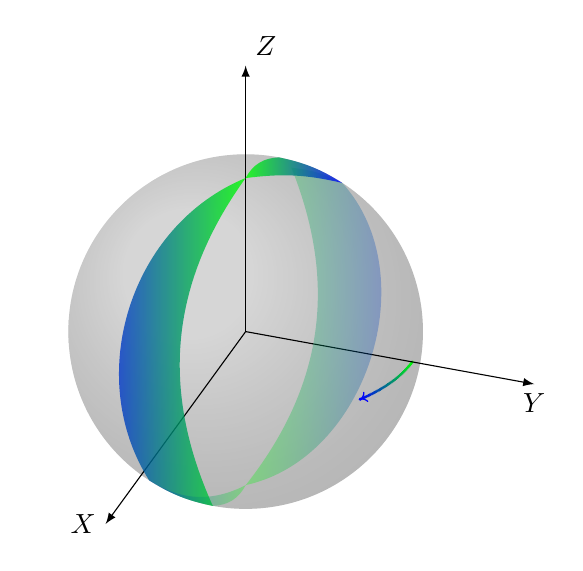
\begin{tikzpicture}[scale=1.3]
		\coordinate (O) at (0,0,0);

		\tdplotsetmaincoords{60}{110}
		\pgfmathsetmacro\R{sqrt(3)}
		\fill[ball color=white!10, opacity=0.2, name path global=C] (O) circle (\R); % 3D lighting effect
		\begin{scope}[tdplot_main_coords, shift={(0,0)}]
			\pgfmathsetmacro\R{sqrt(3)}
			\pgfmathsetmacro{\thetavec}{0};
			\pgfmathsetmacro{\phivec}{0};
			\pgfmathsetmacro{\gammav}{0};
			\tdplotsetrotatedcoords{\phivec}{\thetavec}{\gammav};


			\def\angA{90}
			\def\angB{60}
			\pgfmathsetmacro{\ax}{cos(\angA)}
			\pgfmathsetmacro{\ay}{sin(\angA)}
			\pgfmathsetmacro{\z}{0}
			\pgfmathsetmacro{\bx}{cos(\angB)}
			\pgfmathsetmacro{\by}{sin(\angB)}
			\pgfmathsetmacro{\aax}{\R*cos(\angA)}
			\pgfmathsetmacro{\aay}{\R*sin(\angA)}
			\pgfmathsetmacro{\bbx}{\R*cos(\angB)}
			\pgfmathsetmacro{\bby}{\R*sin(\angB)}

			\coordinate (A) at (\aax,\aay,\z);
			\coordinate (B) at (\bbx,\bby,\z);




			\getEquator{\ay}{\z};
			\tdplotsetrotatedcoords{\alphav}{\betav}{\gammav};
			\tdplotdrawarc[tdplot_rotated_coords,color=green, name path global=GF, opacity=0]
			{(0,0)}{\R}{180}{360}{}{};
			\tdplotdrawarc[tdplot_rotated_coords,color=green, name path global=GB, opacity=0]
			{(0,0)}{\R}{0}{180}{}{};

			\tdplotdrawarc[tdplot_rotated_coords,color=yellow, name path=YB, opacity=0]
			{(0,0)}{\R}{90}{180}{}{};

			\getEquator{\by}{\z};
			\tdplotsetrotatedcoords{\alphav}{\betav}{\gammav};
			\tdplotdrawarc[tdplot_rotated_coords,color=blue, name path=BF, opacity=0]
			{(0,0)}{\R}{180}{360}{}{};
			\tdplotdrawarc[tdplot_rotated_coords,color=blue, name path=BB, opacity=0]
			{(0,0)}{\R}{0}{180}{}{};

			\tdplotdrawarc[tdplot_rotated_coords,color=red, name path=RB, opacity=0]
			{(0,0)}{\R}{90}{180}{}{};

			%\draw[color=red] (A) arc (\angA:\angB:\R); 
			\draw[test=0.2mm] (A) arc (\angA:\angB:\R);



			\InterSec{GF}{BF}{F};
			\InterSec{GB}{BB}{B};
			\InterSec{C}{GF}{CG};
			\InterSec{C}{BF}{CB};
			\InterSec{C}{RB}{RC};
			\InterSec{GB}{RB}{RBF};
			\InterSec{YB}{C}{T};

			%\draw[] (F) circle (1pt) node[] {\; \; \tiny F};
			%\draw[] (CG) circle (1pt) node[] {\tiny CG};
			%\draw[] (CB) circle (1pt) node[] {\tiny CB};
			%\draw[] (B) circle (1pt) node[] {\tiny B};
			%\draw[] (RBF) circle (1pt) node[] {\; \; \tiny RBF};
			%\draw[] (T) circle (1pt) node[] {\tiny T};
			%\draw[] (RC) circle (1pt) node[] {\tiny RC};




			%axis
			\coordinate (X) at (4,0,0) ;
			\coordinate (Y) at (0,3,0) ;
			\coordinate (Z) at (0,0,3) ;

			\draw[-latex] (O) -- (X) node[anchor=east] {\; \; $X$};
			\draw[-latex] (O) -- (Y) node[anchor=north] {$Y$};
			\draw[-latex] (O) -- (Z) node[anchor=south west] {$Z$};

			\shade[left color=blue, right color=green, opacity=0.8] (F) to [bend right=50] (CB) to
			[bend right=10] (CG) to [bend left]  (F);
			\shade[left color=blue, right color=green, opacity=0.3] (CB) to [bend right=10] (CG) to
			[bend right]  (B) to [bend left] (CB);

			\shade[left color=green, right color=blue, opacity=0.3] (B) to [bend right=60] (RC) to
			[bend right=10]  (RBF) to [bend left ] (B);
			\shade[left color=green, right color=blue, opacity=0.8] (F) to [bend left=10] (RC) to
			[bend right=10]  (T) to [bend right] (F);

		\end{scope}
	\end{tikzpicture}

\end{center}


\end{document}
